\PassOptionsToPackage{unicode=true}{hyperref} % options for packages loaded elsewhere
\PassOptionsToPackage{hyphens}{url}
%
\documentclass[british,,man,floatsintext]{apa6}
\usepackage{lmodern}
\usepackage{amssymb,amsmath}
\usepackage{ifxetex,ifluatex}
\usepackage{fixltx2e} % provides \textsubscript
\ifnum 0\ifxetex 1\fi\ifluatex 1\fi=0 % if pdftex
  \usepackage[T1]{fontenc}
  \usepackage[utf8]{inputenc}
  \usepackage{textcomp} % provides euro and other symbols
\else % if luatex or xelatex
  \usepackage{unicode-math}
  \defaultfontfeatures{Ligatures=TeX,Scale=MatchLowercase}
\fi
% use upquote if available, for straight quotes in verbatim environments
\IfFileExists{upquote.sty}{\usepackage{upquote}}{}
% use microtype if available
\IfFileExists{microtype.sty}{%
\usepackage[]{microtype}
\UseMicrotypeSet[protrusion]{basicmath} % disable protrusion for tt fonts
}{}
\IfFileExists{parskip.sty}{%
\usepackage{parskip}
}{% else
\setlength{\parindent}{0pt}
\setlength{\parskip}{6pt plus 2pt minus 1pt}
}
\usepackage{hyperref}
\hypersetup{
            pdftitle={An excess of positive results: Comparing the standard Psychology literature with Registered Reports},
            pdfkeywords={Publication bias, Registered Reports, hypothesis testing},
            pdfborder={0 0 0},
            breaklinks=true}
\urlstyle{same}  % don't use monospace font for urls
\usepackage{graphicx,grffile}
\makeatletter
\def\maxwidth{\ifdim\Gin@nat@width>\linewidth\linewidth\else\Gin@nat@width\fi}
\def\maxheight{\ifdim\Gin@nat@height>\textheight\textheight\else\Gin@nat@height\fi}
\makeatother
% Scale images if necessary, so that they will not overflow the page
% margins by default, and it is still possible to overwrite the defaults
% using explicit options in \includegraphics[width, height, ...]{}
\setkeys{Gin}{width=\maxwidth,height=\maxheight,keepaspectratio}
\setlength{\emergencystretch}{3em}  % prevent overfull lines
\providecommand{\tightlist}{%
  \setlength{\itemsep}{0pt}\setlength{\parskip}{0pt}}
\setcounter{secnumdepth}{0}
% Redefines (sub)paragraphs to behave more like sections
\ifx\paragraph\undefined\else
\let\oldparagraph\paragraph
\renewcommand{\paragraph}[1]{\oldparagraph{#1}\mbox{}}
\fi
\ifx\subparagraph\undefined\else
\let\oldsubparagraph\subparagraph
\renewcommand{\subparagraph}[1]{\oldsubparagraph{#1}\mbox{}}
\fi

% set default figure placement to htbp
\makeatletter
\def\fps@figure{htbp}
\makeatother

\usepackage{etoolbox}
\makeatletter
\providecommand{\subtitle}[1]{% add subtitle to \maketitle
  \apptocmd{\@title}{\par {\large #1 \par}}{}{}
}
\makeatother
% Manuscript styling
\usepackage{csquotes}
\usepackage{upgreek}
\captionsetup{font=singlespacing,justification=justified}

% Table formatting
\usepackage{longtable}
\usepackage{lscape}
% \usepackage[counterclockwise]{rotating}   % Landscape page setup for large tables
\usepackage{multirow}		% Table styling
\usepackage{tabularx}		% Control Column width
\usepackage[flushleft]{threeparttable}	% Allows for three part tables with a specified notes section
\usepackage{threeparttablex}            % Lets threeparttable work with longtable

% Create new environments so endfloat can handle them
% \newenvironment{ltable}
%   {\begin{landscape}\begin{center}\begin{threeparttable}}
%   {\end{threeparttable}\end{center}\end{landscape}}
\newenvironment{lltable}{\begin{landscape}\begin{center}\begin{ThreePartTable}}{\end{ThreePartTable}\end{center}\end{landscape}}

% Enables adjusting longtable caption width to table width
% Solution found at http://golatex.de/longtable-mit-caption-so-breit-wie-die-tabelle-t15767.html
\makeatletter
\newcommand\LastLTentrywidth{1em}
\newlength\longtablewidth
\setlength{\longtablewidth}{1in}
\newcommand{\getlongtablewidth}{\begingroup \ifcsname LT@\roman{LT@tables}\endcsname \global\longtablewidth=0pt \renewcommand{\LT@entry}[2]{\global\advance\longtablewidth by ##2\relax\gdef\LastLTentrywidth{##2}}\@nameuse{LT@\roman{LT@tables}} \fi \endgroup}

% \setlength{\parindent}{0.5in}
% \setlength{\parskip}{0pt plus 0pt minus 0pt}

% Overwrite redefinition of paragraph and subparagraph by the default LaTeX template
% See https://github.com/crsh/papaja/issues/292
\makeatletter
\renewcommand{\paragraph}{\@startsection{paragraph}{4}{\parindent}%
  {0\baselineskip \@plus 0.2ex \@minus 0.2ex}%
  {-1em}%
  {\normalfont\normalsize\bfseries\itshape\typesectitle}}

\renewcommand{\subparagraph}[1]{\@startsection{subparagraph}{5}{1em}%
  {0\baselineskip \@plus 0.2ex \@minus 0.2ex}%
  {-\z@\relax}%
  {\normalfont\normalsize\itshape\hspace{\parindent}{#1}\textit{\addperi}}{\relax}}
\makeatother

% \usepackage{etoolbox}
\makeatletter
\patchcmd{\HyOrg@maketitle}
  {\section{\normalfont\normalsize\abstractname}}
  {\section*{\normalfont\normalsize\abstractname}}
  {}{\typeout{Failed to patch abstract.}}
\makeatother
\shorttitle{Positive Results in Standard vs Registered Reports}
\author{Anne M. Scheel\textsuperscript{1}, Mitchell Schijen\textsuperscript{1}, \& Daniël Lakens\textsuperscript{1}}
\affiliation{
\vspace{0.5cm}
\textsuperscript{1} Eindhoven University of Technology}
\authornote{

Correspondence concerning this article should be addressed to Anne M. Scheel, Den Dolech 1, Atlas 9.417, 5600 MB, Eindhoven, The Netherlands. E-mail: a.m.scheel@tue.nl}
\keywords{Publication bias, Registered Reports, hypothesis testing}
\usepackage{lineno}

\linenumbers
\usepackage{float}
\usepackage{framed}
\usepackage{caption}
\usepackage{setspace}
\captionsetup[figure]{font={stretch=1, small}, skip=10pt}
\captionsetup[textbox]{name=Box,labelsep=period,labelfont=it}
\newfloat{textbox}{thp}{lop}
\floatname{textbox}{Box}
\ifnum 0\ifxetex 1\fi\ifluatex 1\fi=0 % if pdftex
  \usepackage[shorthands=off,main=british]{babel}
\else
  % load polyglossia as late as possible as it *could* call bidi if RTL lang (e.g. Hebrew or Arabic)
  \usepackage{polyglossia}
  \setmainlanguage[variant=british]{english}
\fi

\title{An excess of positive results: Comparing the standard Psychology literature with Registered Reports}

\date{}

\abstract{
Selectively publishing results that support the tested hypotheses (`positive' results) distorts the available evidence for scientific claims. For the past decade, psychological scientists have been increasingly concerned about the degree of such distortion in their literature. A new publication format has been developed to prevent selective reporting: In Registered Reports, peer review and the decision to publish take place before results are known. We compared the results in published Registered Reports (N = 71 as of November 2018) with a random sample of hypothesis-testing studies from the standard literature (N = 152) in Psychology. Analysing the first hypothesis of each paper, we found \(96\%\) positive results in standard reports, but only \(44\%\) positive results in Registered Reports. We discuss possible explanations for this large difference and suggest that a plausible factor is the reduction of publication bias and/or Type-1 error inflation in the Registered-Reports literature.
}

\begin{document}
\maketitle

If the scientific literature were a faithful representation of the research scientists conduct, a cumulative science would be a powerful tool to infer what is true about the world.
When random error is the only threat to the accuracy of individual findings, aggregating across many findings allows inferences about the presence and size of effects with a certain reliability.
But when published findings are systematically biased, cumulative science breaks down:
Unlike random error, bias does not cancel out when aggregating across studies\(\,\)---\(\,\)in the worst case it accumulates, leading us away from the truth rather than towards it.
Unfortunately, there is reason to believe that the Psychology literature is not a faithful representation of all research psychologists conduct.

Since the 1950s, scientists have repeatedly noted a suspiciously high \enquote{success} rate in Psychology:
Studying 362 empirical articles published in four Psychology journals in 1955/56, Sterling (1959) found that \(97.28\%\) of studies using significance tests rejected the null hypothesis.
A later replication of this study reported \(95.56\%\) statistically significant results in articles from 1986/87 (Sterling, Rosenbaum, \& Weinkam, 1995).
Similarly, a seminal study by Fanelli (2010) compared the literatures of 20 disciplines and found that \(91.5\%\) of papers published in Psychology reported support for their first hypothesis, the highest estimate of all disciplines in the study.
For these percentages to be a realistic representation of the research psychologists conduct, both statistical power and the proportion of true hypotheses (i.e., the prior probability that the null hypothesis is false) that are tested must exceed \(90\%\).
Put differently, nearly all predictions researchers make must be correct, and either the studied effects or the used samples (given the same design) must consistently be very large.
These two assumptions appear highly implausible a priori, and available evidence on average statistical power in the literature shows that at least one does not hold (e.g., Szucs \& Ioannidis, 2017).

\hypertarget{a-biased-literature}{%
\subsection{A biased literature}\label{a-biased-literature}}

A more plausible explanation for these numbers may be a selection bias towards statistically significant results in the published literature.
We can distinguish two broad categories of bias: \enquote{publication bias} and \enquote{questionable research practices}.
Publication bias describes publishing behaviours that give manuscripts which find support for their tested hypotheses a higher chance of being published than manuscripts with \enquote{negative} results.
These include editors and reviewers selectively rejecting manuscripts with negative results (``reviewer bias'', Greenwald, 1975; Mahoney, 1977) and researchers deciding not to submit studies with negative results for publication (``file-drawering''; Rosenthal, 1979).
Questionable research practices (QRPs) describe research behaviours that make evidence in favour of a certain conclusion look stronger than it is (typically, though not always, leading to more false positives; see Lakens, 2019).
These include presenting unexpected results as having been predicted \emph{a priori} (HARKing, short for ``hypothesising after results are known''; Kerr, 1998) and exploiting flexibility in data analysis to obtain statistically significant results (``\emph{p}-hacking''; Simmons, Nelson, \& Simonsohn, 2011).
Evidence for both categories of bias exist:
Publication bias has been observed in peer review (Atkinson, Furlong, \& Wampold, 1982; Mahoney, 1977) and in longitudinal data from an NSF grant programme that found a file-drawering effect for studies with negative results (Franco, Malhotra, \& Simonovits, 2014, 2016); and QRPs have been admitted by scientists in several survey studies (Agnoli, Wicherts, Veldkamp, Albiero, \& Cubelli, 2017; Fiedler \& Schwarz, 2016; Fraser, Parker, Nakagawa, Barnett, \& Fidler, 2018; John, Loewenstein, \& Prelec, 2012; Makel, Hodges, Cook, \& Plucker, 2019).

Some have argued that selecting for positive results is defensible\(\,\)---\(\,\)desirable, even\(\,\)---\(\,\)because it weeds out low-quality research that would only pollute the literature (e.g., Cleophas \& Cleophas, 1999).
If most negative results that are currently missing from the literature are indeed due to immature ideas or poor methods, a literature that selects studies based on \emph{quality} instead of results should contain a similar proportion of positive results as the current one.
How many positive and negative results would such an unbiased literature contain in reality?
We investigated this question by comparing the rate of positive results in the Psychology literature to studies published in a new format designed to minimise publication bias and QRPs: Registered Reports.

\hypertarget{methods-to-mitigate-bias}{%
\subsection{Methods to mitigate bias}\label{methods-to-mitigate-bias}}

An increasingly popular proposal to reduce bias is preregistration, where authors register a time-stamped protocol of their hypotheses, methods, and analysis plan before data collection (for a historical overview, see Wiseman, Watt, \& Kornbrot, 2019).
Preregistration is thought to mitigate QRPs by preventing HARKing (hypotheses must be stated before results are known) and by reducing the risk of \emph{p}-hacking via restricted flexibility in data analysis.
However, preregistration does not prevent file-drawering or reviewer bias and may thus be insufficient to fight publication bias (Goldacre et al., 2016; Rasmussen, Lee, \& Bero, 2009; but see Kaplan \& Irvin, 2015).
A more effective safeguard against both publication bias and QRPs is promised by Registered Reports (Chambers \& Tzavella, 2020).

Registered Reports (RRs) are a publication format with a restructured submission timeline:
Before collecting data, authors submit a study protocol containing their hypotheses, planned methods, and analysis pipeline, which undergoes peer review.
If successful, the journal commits to publishing the final article following data collection, regardless of whether the hypotheses are supported (\enquote{in-principle acceptance}).
The authors then collect and analyse the data and complete the final report.
The final report is peer-reviewed again, but this time only to ensure that the the registered plan was adhered to and stated conclusions are justified (and, if applicable, that the data pass pre-specified quality checks).
Registered Reports thus combine an antidote to QRPs (preregistration) with an antidote to publication bias, because studies are selected for publication before their results are known.
Since its introduction in 2013, the format has rapidly gained popularity and is offered by 256 journals at the time of writing (\url{http://cos.io/rr}).

In addition to reducing bias, Registered Reports are designed to ensure high standards for research quality.
First, pre-data peer review increases the chance that methodological flaws and immature ideas will be identified and addressed before a study is conducted.
Second, authors typically have to include outcome-neutral control conditions that allow verifying data quality once results are in (studies failing these quality checks may be rejected).
And third, many journals offering Registered Reports require that hypothesis tests are planned with high statistical power, reducing the risk of false negatives (e.g., \(90\%\) power for a given effect size of interest\footnote{An overview of the requirements specified by each participating journal is available at \url{https://docs.google.com/spreadsheets/d/1D4_k-8C_UENTRtbPzXfhjEyu3BfLxdOsn9j-otrO870}}).

\hypertarget{the-current-study}{%
\subsection{The current study}\label{the-current-study}}

The goal of our study was to test if Registered Reports in Psychology have a lower positive result rate than articles published in the traditional way (henceforth \enquote{standard reports}, SRs), and to estimate the size of this potential difference.
Because the standards for research quality in Registered Reports are at least equal to ordinary peer review, and the statistical power requirements may exceed those in the standard literature (Maxwell, 2004; Szucs \& Ioannidis, 2017), such a difference would be unlikely to be due to \enquote{failed} studies or false negatives.
Should the positive result rate in Registered Reports be much lower than in the standard literature, it might then indicate that publication bias is not a desirable filter for poorly conducted studies, and that we ought to worry about high-quality negative results we are missing because of it.

We set out to compare all published Registered Reports in Psychology with a new sample of standard reports obtained by replicating Fanelli (2010).
Fanelli searched for articles containing the phrase \enquote{test\(^\ast\) the hypothes\(^\ast\)}, drew a random sample of 150 articles per discipline, and coded if the first hypothesis in each article had been supported or not.
For standard reports we used the same sampling method (restricted to the Psychology discipline), for Registered Reports we relied on a database curated by the Center for Open Science (COS).
We chose this method because Fanelli's 2010 and 2012 studies (both use the same coding method) have been highly influential, and because it can easily be applied to a large set of studies.
Because we expected many more Registered Reports than standard reports to be close replications of earlier studies\(\,\)---\(\,\)and perhaps motivated by scepticism of the original results\(\,\)---\(\,\)we additionally examined the role of replications in our analysis.

In a recent commentary, Allen and Mehler (2019) reported a similar investigation:
With a self-developed coding method, they surveyed the 127 biomedical and Psychology Registered Reports listed in the COS database as of September 2018 and found \(60.5\%\) unsupported hypotheses across all included Registered Reports (counting all hypotheses in each paper).
A major advantage of our study, which was planned around the same time (we were unaware of Allen and Mehler's parallel efforts), is the ability to directly compare Registered Reports with the standard literature.
In addition, we replicate Fanelli (2010) and provide data to evaluate his method: The search term \enquote{test\(^\ast\) the hypothes\(^\ast\)} might introduce selection effects, meaning that results obtained this way may not generalise to hypothesis-testing studies that do not use this phrase.
To this end, we coded the phrases used to introduce hypotheses in Registered Reports, analysed how many of them would have been detected with Fanelli's search term, and compiled a list of alternative search terms to test the generalisability of Fanelli's results in the future.
Finally, we share a rich dataset containing the exact quotes of hypotheses and conclusions on which we based our judgements, as well as detailed descriptions of our sampling and coding procedure (see Appendix).
This allows others to verify (or contest) our results and can hopefully provide an interesting resource for future meta-scientific research.

\hypertarget{methods}{%
\section{Methods}\label{methods}}

After conducting a pilot to test the planned procedure, we preregistered our study (\url{https://osf.io/sy927/}).
Methods and analyses described here were preregistered unless otherwise noted.
Our online materials include an Appendix with fine-grained methodological details and an annotated preregistration document with detailed comparisons to the eventual procedure (\url{https://osf.io/dbhgr}).
Appendix and open dataset also list all measures we collected but do not describe here (all of which were either auxiliary variables to facilitate the coding process or earlier versions of the variables discussed here).

\hypertarget{sample}{%
\subsection{Sample}\label{sample}}

We used the same method as Fanelli (2010) to obtain a new sample of standard reports in Psychology, but restricted year of publication to 2013-2018 to match the sample to the Registered Reports population.
We excluded papers in both groups if they were incomplete, unpublished, or retracted (e.g., meeting abstracts, study protocols without results), if they did not test a hypothesis, or if they contained insufficient information to reach a coding decision.
An overview of the sampling process and all exclusions is shown in Figure~\ref{fig:sampling}.

The sample size of standard reports was pre-specifided to replicate Fanelli's (2010) (\(n = 150\)) since it matched the maximum number of available Registered Reports (\(n = 151\), see below) and piloting indicated that the required coding time would just fit our resource constraints.
Standard reports were selected by searching the 633 journals listed under \enquote{Psychiatry/Psychology} in the Essential Science Indicators database for papers published between 2013 and 2018 that contained the phrase \enquote{test\(^\ast\) the hypothes\(^\ast\)} in title, abstract, or keywords.
We then randomly selected 150 papers from the 1919 papers that resulted from this search. Excluded papers were replaced by resampling twice (this decision was not preregistered), which led to accidental oversampling and a final sample size of 152 (see Fig.~\ref{fig:sampling}).



\begin{figure}
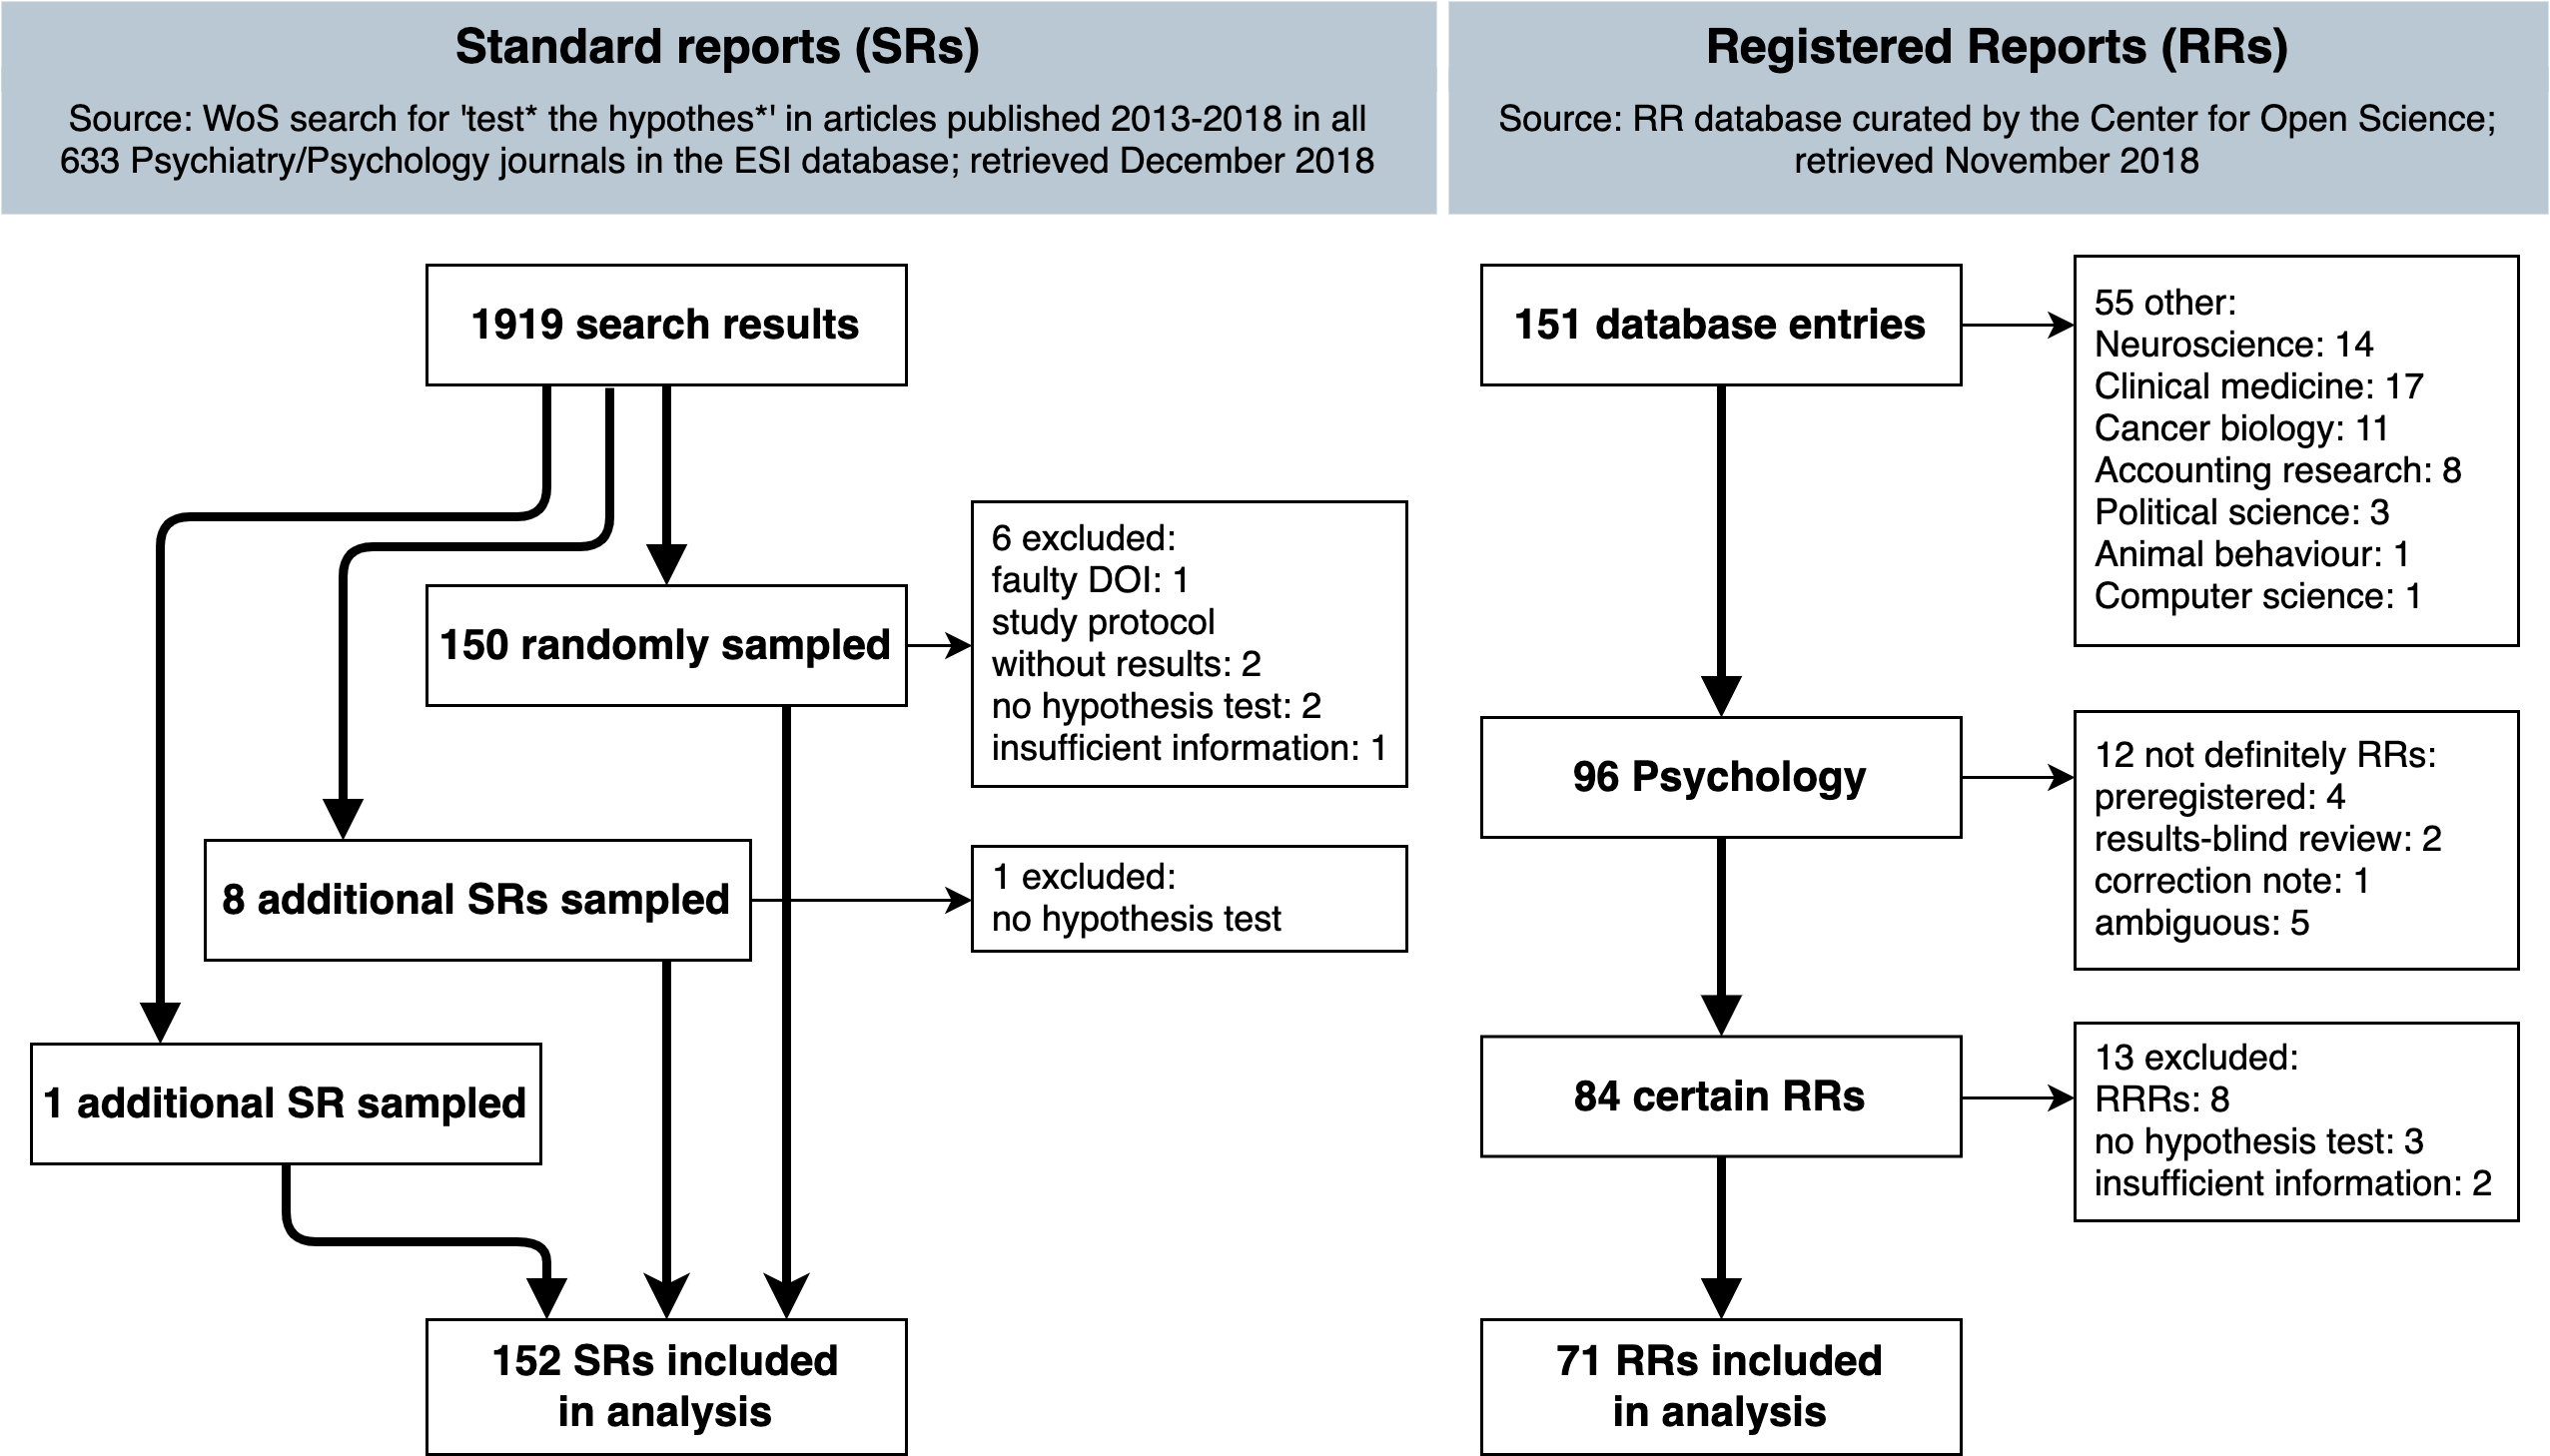
\includegraphics[width=\textwidth]{sampling_process_flowchart} \caption{Sampling process and exclusions for standard reports and Registered Reports. Standard reports were accidentally oversampled: We initially excluded 8 papers and only after replacing them found that two had been excluded erroneously. \enquote{Preregistered}: study had been preregistered but was not a full RR; \enquote{results-blind review}: article had undergone results-blind peer review but was not a full RR (authors knew results before first submission); \enquote{ambiguous}: four of these had been treated as Registered Reports but used pre-existing data to which the authors had access before conducting their analyses, one had no explicit signs of an RR except for a 2.5-year delay between submission and acceptance (we chose to exclude these cases to be conservative).}\label{fig:sampling}
\end{figure}

The sample size of Registered Report was determined by our goal to include all published Registered Reports in the field of Psychology that tested at least one hypothesis, regardless of whether they used the phrase \enquote{test\(^\ast\) the hypothes\(^\ast\)}.
Registered Reports were selected through a Registered-Reports database curated by the Center for Open Science\footnote{\url{https://www.zotero.org/groups/479248/osf/items/collectionKey/KEJP68G9}} (retrieved 19th November 2018).
After excluding non-Psychology papers, we verified that all remaining papers were indeed Registered Reports by consulting the journal submission guidelines, relevant editorials, or contacting the editors directly.
Papers were counted as Registered Reports if we could establish that these submissions had been reviewed and received in-principle acceptance before the data collection (or analyses) of all studies in the paper had been conducted (in accordance with \url{https://cos.io/rr}).
We excluded 80 of the 151 entries in the COS Registered Reports database, leaving 71 Registered Reports for the final analysis (see Fig.~\ref{fig:sampling}).
Note that we excluded all eight \enquote{Registered Replication Reports} (RRRs; Simons, Holcombe, \& Spellman, 2014; Simons, 2018) in our sample because this format explicitly focuses on effect size estimation and not hypothesis testing (``Registered Replication Reports,'' n.d., decision was not preregistered).

\hypertarget{measures-and-coding-procedure}{%
\subsection{Measures and coding procedure}\label{measures-and-coding-procedure}}

The main dependent variable was whether the first hypothesis was supported or not, as reported by the authors.
We tried to follow Fanelli's coding procedure as closely as possible:

\begin{quote}
By examining the abstract and/or full- text, it was determined whether the authors of each paper had concluded to have found a positive (full or partial) or negative (null or negative) support.
If more than one hypothesis was being tested, only the first one to appear in the text was considered.
We excluded meeting abstracts and papers that either did not test a hypothesis or for which we lacked sufficient information to determine the outcome. (Fanelli, 2010, p. 8)
\end{quote}

In Registered Reports, we coded the first \emph{preregistered} hypothesis, thus excluding unregistered pilot studies.
Coding disagreements between \enquote{full} and \enquote{partial} support were deemed minor since they would not affect the final results.
Thus, only disagreements affecting the binary support (full or partial) vs no support classification were treated as major and resolved through discussion.
MS coded all papers in the sample, AS double-coded all papers MS had found difficult to code or could not code (\(24\) RRs and \(47\) SRs).
Only 3 disagreements were major (Cohen's kappa = .808) and subsequently resolved by discussion; 15 were minor (disagreement between \enquote{support} and \enquote{partial support}).
We overturned the preregistered plan that AS would additionally code a random subset of both groups, because the number of double-coded papers seemed sufficient after double-coding only the difficult cases.
Coders were not blind to condition (Registered Report vs standard report) because access to the full text was often necessary, the content of which would have made most Registered Reports clearly identifiable.

\hypertarget{hypothesis-introductions}{%
\subsubsection{Hypothesis introductions}\label{hypothesis-introductions}}

Selecting standard reports based on the phrase \enquote{test\(^\ast\) the hypothes\(^\ast\)} might yield different results than alternative search phrases.
To get a better overview of \enquote{natural} descriptions of hypotheses and facilitate future investigations of the generalisability of Fanelli's (2010) results, we extracted the phrase used to introduce the coded hypothesis in all Registered Reports and tried to identify clusters of common expressions.

\hypertarget{replication-status}{%
\subsubsection{Replication status}\label{replication-status}}

We expected a large proportion of Registered Reports to be replications, many of which may have been motivated by scepticism of the original study.
Because this circumstance alone could potentially lead to a lower positive result rate in Registered Reports, we additionally coded if hypotheses were close replications of previously published work.
Due to ill-specified coding criteria in our preregistration (see Appendix), we used an unregistered coding strategy:
We determined whether the coded hypothesis of papers whose full text contained the string \enquote{replic\(^\ast\)} (cf. Makel, Plucker, \& Hegarty, 2012; Mueller-Langer, Fecher, Harhoff, \& Wagner, 2019) was a close replication with the goal to verify a previously published result.
Conceptual replications and internal replications (replication of a study in the same paper) were not counted as replications in this narrow sense, since both are more likely to be motivated by the goal to build on previous work than by scepticism.
AS coded all papers, DL double-coded 32 Registered Reports (\(45.07 \%\)) and 99 standard reports (\(65.13 \%\)).
There were 5 disagreements (Cohen's kappa = .878), all were resolved by discussion.

\hypertarget{analysis}{%
\subsection{Analysis}\label{analysis}}

We planned to test our hypothesis in the following way (quoting directly from our preregistration, \url{https://osf.io/sy927}):

\begin{quote}
A one-sided proportion test with an alpha level of \(5\%\) will be performed to test whether the positive result rate (full or partial support) of Registered Reports in psychology is statistically lower than the positive result rate of conventional reports\footnote{We later changed the term to \enquote{standard reports}.} in psychology.
In addition to testing if there is a statistically significant difference between RRs and conventional reports, we will test if the difference is smaller than our smallest effect size of interest using an equivalence test for proportion tests with an alpha level of \(5\%\) (Lakens, Scheel, \& Isager, 2018).
We determined our smallest effect size of interest to be the difference between the positive result rate in psychology (\(91.5\%\)) and the positive result rate in general social sciences (\(85.5\%\)) as reported by Fanelli (2010), i.e.~a difference of \(91.5\% - 85.5\% = 6\%\).
The rationale for choosing general social sciences as a comparison is that this discipline had the lowest positive result rate amongst the \enquote{soft} sciences (Fanelli, 2010).
The exact percentage for general social sciences was extracted from Figure 1 in Fanelli (2010) using the software WebPlotDigitizer (Rohatgi, 2018).
\end{quote}

We would accept our hypothesis that Registered Reports have a lower positive result rate than standard reports if the observed difference between Registered Reports and standard reports was significantly smaller than 0 \emph{and} not statistically equivalent to a range from \(-6\%\) to \(+6\%\) (both at \(\alpha = 5\%\)).

\hypertarget{results}{%
\section{Results}\label{results}}

\hypertarget{preregistered-analysis}{%
\subsection{Preregistered analysis}\label{preregistered-analysis}}

31 out of 71 Registered Reports and 146 out of 152 standard reports had positive results, meaning that the positive result rate was \(43.66 \%\) for Registered Reports (\(95 \%\) CI {[}31.91, 55.95{]}) and \(96.05 \%\) for standard reports (\(95 \%\) CI {[}91.61, 98.54{]}; see Fig.~\ref{fig:mainplot}).
This difference of \(-52.39 \%\) was statistically significant in the preregistered one-sided proportions test with \(\alpha = 5\%\), \(\chi^2(1) = 77.96\), \(p < .001\).
Unsurprisingly, the difference was not statistically equivalent to a range between \(-6 \%\) and \(6 \%\) at \(\alpha = 5\%\) (\(z = 7.61\), \(p > .999\)), meaning that we cannot reject differences more extreme than \(6\%\).
We thus accept our hypothesis that the positive result rate in Registered Reports is lower than in standard reports.



\begin{figure}
\centering
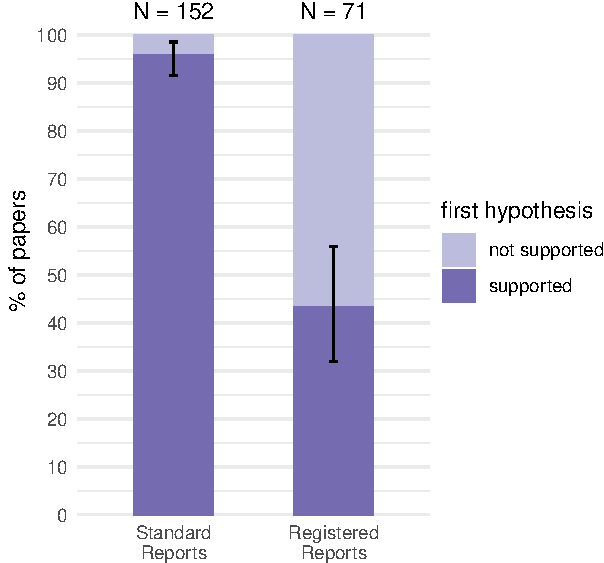
\includegraphics{positive_results_SRs_RRs_revision1_files/figure-latex/mainplot-1.pdf}
\caption{\label{fig:mainplot}Positive result rates for standard reports and Registered Reports. Error bars indicate \(95 \%\) confidence intervals around the observed positive result rate.}
\end{figure}

\hypertarget{exploratory-analyses}{%
\subsection{Exploratory analyses}\label{exploratory-analyses}}

For ease of communication we will refer to papers that were classified as close replications of previously published work as \enquote{replications} and to all other studies as \enquote{original}, even though the latter include some conceptual replications and internal replications (as explained above).
As expected, replications were much more common among Registered Reports (\(41 / 71 = 57.75\%\)) than standard reports (\(4 / 152 = 2.63\%\)), and replication Registered Reports had a descriptively lower positive result rate than original Registered Reports (see Table 1).
However, this finding fails to explain the main result described above:
When analysing only original papers, the difference between the positive result rates of Registered Reports and standard reports, \(-45.95\%\), was still significantly different from 0 (\(\chi^2(1) = 46.28\), \(p < .001\)) and not statistically equivalent to a range between \(-6\%\) and \(6\%\) (\(z = 4.31\), \(p > .999\)), both at \(\alpha = 5\%\).



\begin{table}[tbp]

\begin{center}
\begin{threeparttable}

\caption{\label{tab:unnamed-chunk-4}Positive results in original studies vs replication studies}

\begin{tabular}{lrrrrrrrr}
\toprule
 & \multicolumn{4}{c}{original studies} & \multicolumn{4}{c}{replication studies} \\
\cmidrule(r){2-5} \cmidrule(r){6-9}
 & n & supported & \% & 95\% CI & n & supported & \% & 95\% CI\\
\midrule
SRs & 148 & 142 & 95.95 & 91.39; 98.50 & 4 & 4 & 100.00 & 39.76; 100.00\\
RRs & 30 & 15 & 50.00 & 31.30; 68.70 & 41 & 16 & 39.02 & 24.20; 55.50\\
\bottomrule
\addlinespace
\end{tabular}

\begin{tablenotes}[para]
\normalsize{\textit{Note.} SRs = standard reports, RRs = Registered Reports}
\end{tablenotes}

\end{threeparttable}
\end{center}

\end{table}

Since our standard-reports sample represents a direct replication of Fanelli (2010) for the discipline Psychiatry \& Psychology, another interesting question is how our results compare to Fanelli's.
The difference between the positive result rates of standard reports in our sample and Fanelli's (\(96.05\% - 91.49\% = 4.56\%\)) is not significantly different from 0 in a two-sided proportions test (\(\chi^2(1) = 1.91\), \(p= .167\)) but also not statistically equivalent to a range between \(-6\%\) and \(6\%\) (\(z = 0.51\), \(p= .306\)), both at \(\alpha = 5\%\).
The data are inconclusive:
We can neither reject the hypothesis that the positive result rates of the two populations are the same, nor that there is a difference of at least \(\pm 6\%\) between them.

Finally, we analysed the language that was used to introduce or refer to hypotheses in Registered Reports.
We found extremely little overlap with Fanelli's search phrase \enquote{test\(^\ast\) the hypothes\(^\ast\)}:
Searching the abstracts, titles, and keywords of the Registered Reports sample showed that only 2/71 Registered Reports would have been detected with this search phrase.
To analyse which other hypothesis-introduction phrases researchers used in Registered Reports, we stripped the coded hypothesis quotes from all content-specific information and extracted \enquote{minimal} phrases that most distinctively indicated that a hypothesis was being described.
For example, from the hypothesis quote \enquote{(f)or Study 1, we predicted that participants reading about academic (vs.~social) behaviors would show a better anagram performance} we extracted the hypothesis-introduction phrase \enquote{predicted that}.

For the majority of Registered Reports (49), we identified one hypothesis-introduction phrase; the remaining ones used two (16 RRs), three (4 RRs), or four (1 RR) different phrases or had no identifiable hypothesis introduction (1 RR).
In this total set of 97 hypothesis introductions, we found 64 unique phrases showing substantial linguistic variation (see Tables 2 and 3).
We then listed all unique word stems within those phrases and analysed their frequency.
Excluding words that are common but too unspecific by themselves (e.g., \enquote{that}, \enquote{to}, \enquote{whether}), the five most frequent word stems were \enquote{hypothes\(^\ast\)} (34 occurrences), \enquote{replicat\(^\ast\)} (24), \enquote{test\(^\ast\)} (20), \enquote{examine\(^\ast\)} (8), and \enquote{predict\(^\ast\)} (8).
Clearly, \enquote{test\(^\ast\)} and \enquote{hypothes\(^\ast\)} are quite popular, yet they co-occurred only 8 times, and more than half of all hypothesis introductions (51/97) contained neither word.

69 of the 71 Registered Reports (\(97.18 \%\)) had at least one of these five most frequent word stems in their title, abstract, or keywords, meaning that a regular literature search (without access to full texts) with the search terms \enquote{hypothes\(^\ast\) \emph{OR} replicat\(^\ast\) \emph{OR} test\(^\ast\) \emph{OR} examine\(^\ast\) \emph{OR} predict\(^\ast\)} would have been effective in identifying these papers.
We do not know how well these search terms represent the population of hypothesis-testing studies in Psychology, but a structured investigation of this question could be useful for future meta-research.

Lastly, we noticed an interesting difference in language use between original and replication Registered Reports:
As the high frequency of the word stem \enquote{replicat\(^\ast\)} suggests, replications were often framed as attempts to repeat a previously conducted \emph{procedure} rather than as attempts to test a previously tested \emph{hypothesis}.
Tables 2 and 3 list all unique hypothesis introductions and their frequency in original Registered Reports and replication Registered Reports, respectively, grouped by the five most frequent word stems (\enquote{hypothes\(^\ast\)}, \enquote{replicat\(^\ast\)}, \enquote{test\(^\ast\)}, \enquote{examine\(^\ast\)}, \enquote{predict\(^\ast\)}).



\begin{table}[tbp]

\begin{center}
\begin{threeparttable}

\caption{\label{tab:unnamed-chunk-6}Hypothesis introduction phrases in original Registered Reports (testing new hypotheses)}

\scriptsize{

\begin{tabular}{llrrr}
\toprule
 &  & \multicolumn{3}{c}{source} \\
\cmidrule(r){3-5}
core word(s) & introduction phrase & abstract & full text & total\\
\midrule
hypothes* &  & 5 & 12 & 17\\
 & (Hypothesis 1) & 0 & 1 & 1\\
 & Hypothesis 1 (H1): & 0 & 2 & 2\\
 & Hypothesis 1: & 0 & 1 & 1\\
 & Hypothesis 1a (H1a): & 0 & 1 & 1\\
 & hypothesis was & 0 & 1 & 1\\
 & Hypothesis: & 0 & 1 & 1\\
 & hypothesize that & 0 & 3 & 3\\
 & hypothesized that & 4 & 2 & 6\\
 & registered ... hypotheses & 1 & 0 & 1\\ \midrule
hypothes*, test* &  & 3 & 2 & 5\\
 & test of ... hypotheses & 0 & 1 & 1\\
 & test of ... hypothesis & 1 & 0 & 1\\
 & test the hypothesis that & 1 & 0 & 1\\
 & tested ... hypotheses & 0 & 1 & 1\\
 & tested the hypothesis that & 1 & 0 & 1\\ \midrule
test* &  & 5 & 2 & 7\\
 & test if & 0 & 1 & 1\\
 & test whether & 1 & 1 & 2\\
 & tested whether & 2 & 0 & 2\\
 & testing & 1 & 0 & 1\\
 & to ... test & 1 & 0 & 1\\ \midrule
test*, predict* & test ... prediction & 0 & 1 & 1\\ \midrule
examin* &  & 5 & 0 & 5\\
 & examine whether & 2 & 0 & 2\\
 & examined & 1 & 0 & 1\\
 & examined whether & 1 & 0 & 1\\
 & to examine & 1 & 0 & 1\\ \midrule
predict* &  & 4 & 0 & 4\\
 & had ... predictions & 1 & 0 & 1\\
 & predicted that & 2 & 0 & 2\\
 & predicts that & 1 & 0 & 1\\ \midrule
(other) &  & 0 & 5 & 5\\
 & (H1) & 0 & 1 & 1\\
 & expected that & 0 & 1 & 1\\
 & if ... then & 0 & 1 & 1\\
 & predication that & 0 & 1 & 1\\
 & we expect & 0 & 1 & 1\\
\bottomrule
\addlinespace
\end{tabular}

}

\begin{tablenotes}[para]
\normalsize{\textit{Note.} Table contains 44 hypothesis introduction phrases from 30 Registered Reports: 19 papers contributed one phrase each, nine papers contributed two each, one contributed three, and one contributed four.}
\end{tablenotes}

\end{threeparttable}
\end{center}

\end{table}



\begin{table}[tbp]

\begin{center}
\begin{threeparttable}

\caption{\label{tab:unnamed-chunk-7}Hypothesis introduction phrases in direct replication Registered Reports (testing previously studied hypotheses)}

\scriptsize{

\begin{tabular}{lllrrrr}
\toprule
 &  &  & \multicolumn{3}{c}{source}  &\\
\cmidrule(r){4-6}
 & core word(s) & introduction phrase & abstract & full text & total & \\
\midrule
 & hypothes* &  & 2 & 5 & 7 & \\
 &  & according to ... hypothesis & 0 & 1 & 1 & \\
 &  & Hypotheses & 0 & 1 & 1 & \\
 &  & Hypothesis 1 (H1): & 0 & 1 & 1 & \\
 &  & hypothesize that & 0 & 1 & 1 & \\
 &  & hypothesized that & 2 & 1 & 3 & \\ \midrule
 & hypothes*, test* &  & 2 & 1 & 3 & \\
 &  & test ... hypotheses & 0 & 1 & 1 & \\
 &  & test ... hypothesis & 1 & 0 & 1 & \\
 &  & tested ... hypotheses & 1 & 0 & 1 & \\ \midrule
 & hypothes*, examin* & examined ... hypothesis & 1 & 0 & 1 & \\ \midrule
 & hypothes*, predict* & hypotheses predicted & 1 & 0 & 1 & \\ \midrule
 & replicat* &  & 20 & 3 & 23 & \\
 &  & aim ... to replicate & 0 & 1 & 1 & \\
 &  & aim at replicating & 1 & 0 & 1 & \\
 &  & aimed to replicate & 0 & 1 & 1 & \\
 &  & attempted to replicate & 1 & 0 & 1 & \\
 &  & attempts to replicate & 1 & 0 & 1 & \\
 &  & conducted ... replication & 3 & 0 & 3 & \\
 &  & conducted ... replications & 2 & 0 & 2 & \\
 &  & performed ... replication & 2 & 0 & 2 & \\
 &  & present ... replication & 1 & 0 & 1 & \\
 &  & present ... replications & 1 & 0 & 1 & \\
 &  & replicated ... experiment & 1 & 0 & 1 & \\
 &  & replicating & 0 & 1 & 1 & \\
 &  & report ... replication attempt & 1 & 0 & 1 & \\
 &  & report ... replications & 2 & 0 & 2 & \\
 &  & sought to replicate & 3 & 0 & 3 & \\
 &  & we replicated & 1 & 0 & 1 & \\ \midrule
 & replicat*, examin* & critically examine and replicate & 1 & 0 & 1 & \\ \midrule
 & test* &  & 4 & 0 & 4 & \\
 &  & testing whether & 2 & 0 & 2 & \\
 &  & to ... test & 1 & 0 & 1 & \\
 &  & to test & 1 & 0 & 1 & \\ \midrule
 & examin* & examine whether & 0 & 1 & 1 & \\ \midrule
 & predict* & predicted that & 2 & 0 & 2 & \\ \midrule
 & (other) &  & 4 & 6 & 10 & \\
 &  & establish whether & 0 & 1 & 1 & \\
 &  & H1 & 0 & 2 & 2 & \\
 &  & investigate if & 1 & 0 & 1 & \\
 &  & sought to reproduce & 1 & 0 & 1 & \\
 &  & suggests that & 2 & 0 & 2 & \\
 &  & we ... conducted & 0 & 1 & 1 & \\
 &  & we assume & 0 & 1 & 1 & \\
 &  & we expect & 0 & 1 & 1 & \\
\bottomrule
\addlinespace
\end{tabular}

}

\begin{tablenotes}[para]
\normalsize{\textit{Note.} Table contains 53 hypothesis introduction phrases from 40 Registered Reports. One additional RR had no identifiable hypothesis introduction. Thirty papers contributed one phrase each, seven contributed two each, and three contributed three each.}
\end{tablenotes}

\end{threeparttable}
\end{center}

\end{table}

\hypertarget{discussion}{%
\section{Discussion}\label{discussion}}

We examined the proportion of Psychology articles that find support for their first tested hypothesis and discovered a large difference (\(96.05 \%\) vs \(43.66 \%\)) between a random sample of standard reports and the full population of Registered Reports (at the time of data collection).
More than half of the analysed hypothesis tests in Registered Reports were close replications of previous work, but the difference between standard reports and Registered Reports remained large when close replications were excluded from the analysis (\(95.95 \%\) vs \(50.00 \%\)).
Clearly, the emerging literature of Registered Reports appears to be publishing a much larger proportion of null results than the standard literature.

The positive result rate we found in standard reports (\(96.05 \%\)) is slightly but non-significantly higher than the \(91.5\%\) reported by Fanelli (2010).
Our replication in a more recent sample of the Psychology literature thus yielded a comparably high estimate of supported hypotheses, but we cannot rule out that the positive result rate in the population has increased since 2010 (cf. Fanelli, 2012).
Furthermore, our estimate of the positive result rate for Registered Reports (\(43.66 \%\)) is comparable to the \(39.5\%\) reported by Allen and Mehler (2019), despite some differences in method and studied population.

To explain the \(52.39 \%\) gap between standard reports and Registered Reports, we must assume some combination of differences in bias, statistical power, or the proportion of true hypotheses researchers choose to examine.
Figure~\ref{fig:powerbaserate} visualises the combinations of statistical power and proportion of true hypotheses that could produce the observed positive result rates if the literature were completely unbiased.
Assuming no publication bias and no QRPs, authors of standard reports would need to test almost exclusively true hypotheses (\(>90\%\)) with more than \(90\%\) power.
Because this is highly implausible and contradicted by available evidence (e.g., Szucs \& Ioannidis, 2017), the standard literature is unlikely to reflect reality.
As noted above, methodological rigour and statistical power in Registered Reports likely meet or exceed the level of standard reports, leaving the rate of true hypotheses and bias as remaining explanations.



\begin{figure}

{\centering 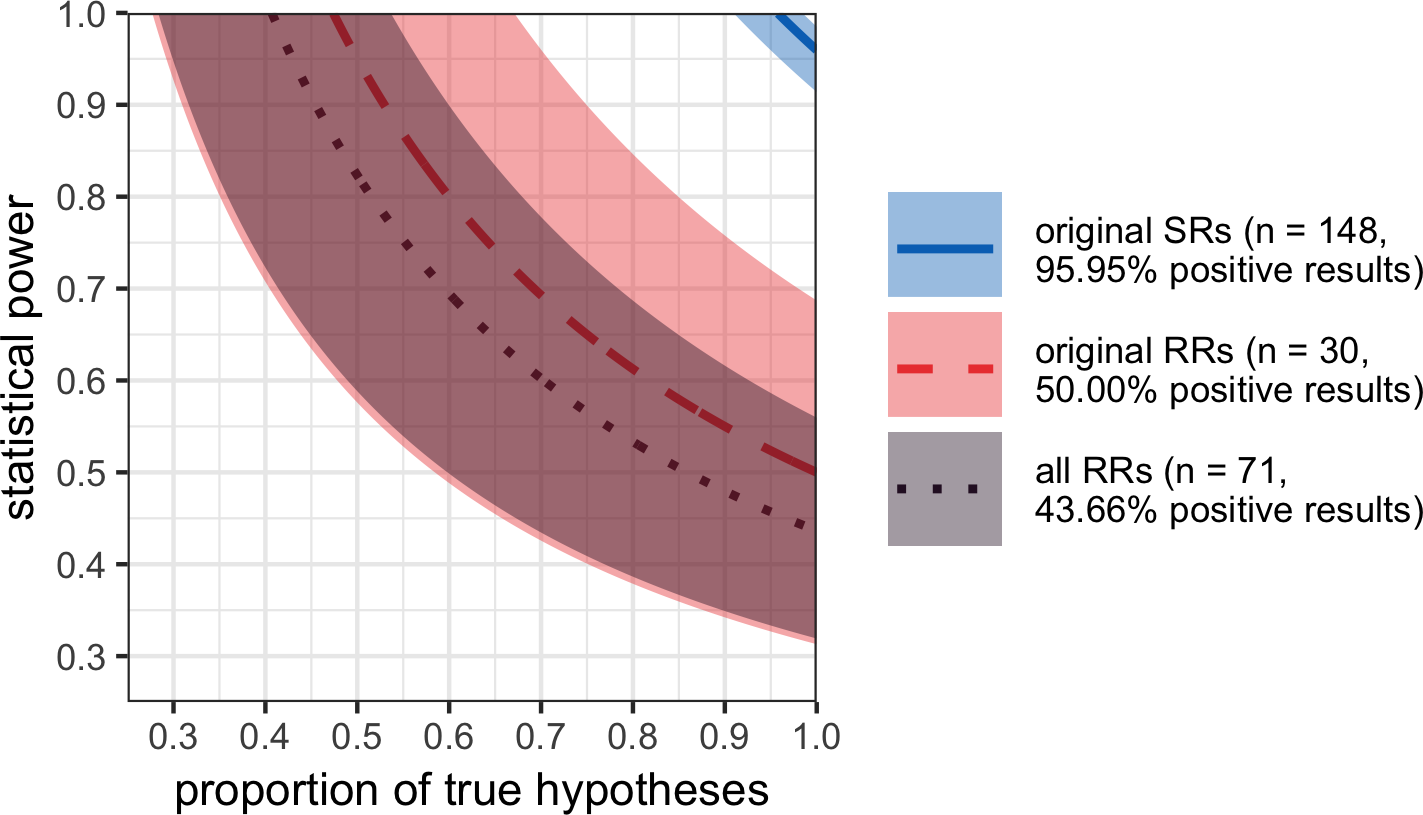
\includegraphics[width=0.8\textwidth]{positive_results_SRs_RRs_revision1_files/figure-latex/powerbaserate-1} 

}

\caption{Combinations of the proportion of true hypotheses and statistical power that would produce the observed positive result rates given \(\alpha = 5 \%\) and no bias. Shaded areas indicate \(95\%\) confidence intervals. SRs = standard reports, RRs = Registered Reports. The curve for all SRs (i.e, including replications; \(96.05 \%\) positive results, \(N = 152\)) is not shown because it is almost identical to the one for original SRs. Plotted values were calculated using the equation \(PRR = \alpha*(1-t) + (1-\beta)*t\); with \(PRR =\) positive result rate, \(\alpha =\) probability of obtaining a positive result when testing a false hypothesis (here fixed at .05), \(1-\beta =\) probability of obtaining a positive result when testing a true hypothesis (power), and \(t =\) proportion of true hypotheses; and solving for \(t\) and \(1-\beta\), respectively (with the simplifying assumption that all studies in one group have the same power).}\label{fig:powerbaserate}
\end{figure}

It is \emph{a-priori} plausible that Registered Reports are currently used for a population of hypotheses that are less likely to be true:
For example, authors may use the format strategically for studies they expect to yield negative results (which would be difficult to publish otherwise).
However, assuming over \(90\%\) true hypotheses in the standard literature is neither realistic, nor would it be desirable for a science that wants to advance knowledge beyond trivial facts.
We thus believe that this factor alone is not sufficient to explain the large difference in positive results.
Rather, the numbers strongly suggest a reduction of publication bias and/or QRPs in the Registered-Reports literature.
Nonetheless, the prior probability of hypotheses in Registered Reports and standard reports may differ and should be studied in future research.

\hypertarget{limitations}{%
\subsection{Limitations}\label{limitations}}

Our study was not an experiment\(\,\)---\(\,\)hypotheses, authors, and editors were not randomly assigned to each publication format\(\,\)---\(\,\)and thus precludes strong causal inferences.
As discussed above, it seems highly plausible that Registered Reports reduce publication bias and QRPs, which in turn reduces the positive result rate.
Yet we neither know exactly how effective Registered Reports are at reducing bias, nor how large the effect on positive results would be in the absence of potential confounds.
One such confound, as just discussed, could be that Registered Reports may be used for particularly risky hypotheses.
Another confound could be that the format attracts particularly conscientious authors who try to minimise the risk of inflated error rates regardless of the report format they use.
This would lead to less bias in the Registered-Reports literature even if the format's safeguards against certain QRPs were actually ineffective.

Another limitation of the current study (and of Fanelli, 2010) is that standard reports were selected using the search phrase \enquote{test\(^\ast\) the hypothes\(^\ast\)}.
This phrase was virtually absent in Registered Reports, suggesting that the search strategy may not yield a representative sample of the population of hypothesis-testing studies in the literature.
The use of the phrase might even be confounded with the outcome of a study:
For example, authors may be more likely to describe their research explicitly as a hypothesis test when they found positive results, but prefer more vague language for unsupported hypotheses (e.g., \enquote{we examined the role of \ldots{}}).
A similar concern could be raised for the decision to code only the first reported hypothesis of each article.
The first hypothesis test may not be representative for all hypothesis tests reported in a paper, and the order of reporting may differ between standard reports and Registered Reports.
For example, standard-report authors might tend to present supported hypotheses first, whereas Registered-Report authors might be more likely to present their hypotheses in \enquote{chronological} order.

Both of these potential confounds might lead to an inflated estimate of the positive result rate in standard reports.
However, studies using different selection criteria for articles and hypotheses have found very similar rates of supported hypotheses in the literature:
\(97.28\%\) in Sterling (1959), \(95.56\%\) in Sterling et al. (1995), and \(97\%\) in the original studies included in the Reproducibility Project: Psychology (Open Science Collaboration, 2015).
In addition, Motyl et al. (2017) report \(89.17\%\) and \(92.01\%\) significant results for \enquote{critical} hypothesis tests in papers published in 2003-2004 and 2013-2014, respectively.
Although the selection criteria for articles and hypotheses in our study may limit the generalisability of the results, this level of convergence makes it seem unlikely that alternative methods would have yielded dramatically different conclusions.

\hypertarget{conclusion}{%
\subsection{Conclusion}\label{conclusion}}

Our study presents a systematic comparison of positive results in Registered Reports and the standard literature. The much lower positive result rate in Registered Reports compared to standard reports suggests that an unbiased literature would look very different from the existing body of published research. Standard publication formats seem to lead psychological scientists to miss out on many negative results from high-quality studies, which are available in the Registered-Reports literature. The absence of negative results is a serious threat to a cumulative science. In 1959, Sterling asked: \enquote{What credence can then be given to inferences drawn from statistical tests of \(H_0\) if the reader is not aware of all experimental outcomes of a kind?} The amount of experimental outcomes missing from the standard literature appears to be so large that not much credence may be left. In contrast, Registered Reports have clearly led to a much larger proportion of negative results appearing in the literature\(\,\)---\(\,\)and may be one solution to achieve a more credible scientific record.

\hypertarget{disclosures}{%
\subsection{Disclosures}\label{disclosures}}

\hypertarget{data-materials-and-online-resources}{%
\subsubsection{Data, materials, and online resources}\label{data-materials-and-online-resources}}

\href{https://osf.io/aqr2s/}{Data} and code necessary to reproduce all analyses reported here, as well as the \href{https://osf.io/qw798/}{Appendix}, the \href{https://osf.io/sy927/}{preregistration}, and additional supplementary files, are available at \url{https://osf.io/dbhgr}.
The manuscript, including figures and statistical analyses, the \href{https://osf.io/qw798/}{Appendix}, and the \href{https://osf.io/6jrkz/}{codebook} available in the supplement were created using RStudio (1.2.5019, RStudio Team, 2019) and R (Version 3.6.0; R Core Team, 2019) and the R-packages \emph{bookdown} (Version 0.17; Xie, 2016), \emph{codebook} (Version 0.8.2; Arslan, 2018), \emph{ggplot2} (Version 3.1.1; Wickham, 2016), \emph{here} (Version 0.1; Müller, 2017), \emph{knitr} (Version 1.26; Xie, 2015), \emph{papaja} (Version 0.1.0.9842; Aust \& Barth, 2018), \emph{reshape2} (Version 1.4.3; Wickham, 2007), \emph{rio} (Version 0.5.16; Chan, Chan, Leeper, \& Becker, 2018), \emph{rmarkdown} (Version 1.18; Xie, Allaire, \& Grolemund, 2018), \emph{stringr} (Version 1.4.0; Wickham, 2019), and \emph{TOSTER} (Version 0.3.4; Lakens, 2017).

\hypertarget{reporting}{%
\subsubsection{Reporting}\label{reporting}}

We report how we determined our sample size, all data exclusions, all manipulations, and all measures in the study.

\hypertarget{author-contributions}{%
\subsubsection{Author Contributions}\label{author-contributions}}

Conceptualisation: A.S. \& D.L.; data curation, formal analysis, and software: A.S. \& M.S.; investigation, methodology, and validation: A.S., M.S., \& D.L; supervision: A.S \& D.L.; visualisation and writing\(\,\)---\(\,\)original draft: A.S; writing\(\,\)---\(\,\)review and editing: A.S., M.S., \& D.L.

\hypertarget{conflicts-of-interest}{%
\subsubsection{Conflicts of Interest}\label{conflicts-of-interest}}

The authors declare that they have no conflicts of interest with respect to the authorship or the publication of this article.

\hypertarget{acknowledgements}{%
\subsubsection{Acknowledgements}\label{acknowledgements}}

This work was funded by VIDI grant 452-17-013. We thank Chris Chambers, Emma Henderson, Leonid Tiokhin, and Stuart Ritchie for valuable comments that helped improve this manuscript.

\hypertarget{prior-versions}{%
\subsubsection{Prior versions}\label{prior-versions}}

A preprint of this manuscript has been published on \emph{PsyArXiv} (\url{https://doi.org/10.31234/osf.io/p6e9c}). All sections of the present manuscript have been shortened to comply with the submission guidelines, but are intended to contain the same arguments, methods, results, and conclusions as the preprint.

\hypertarget{references}{%
\section{References}\label{references}}

\setlength{\parindent}{-0.2in}
\setlength{\leftskip}{0.2in}

\hypertarget{refs}{}
\leavevmode\hypertarget{ref-Agnoli2017}{}%
Agnoli, F., Wicherts, J. M., Veldkamp, C. L. S., Albiero, P., \& Cubelli, R. (2017). Questionable research practices among italian research psychologists. \emph{PLOS ONE}, \emph{12}(3), e0172792. \url{https://doi.org/10.1371/journal.pone.0172792}

\leavevmode\hypertarget{ref-Allen2019}{}%
Allen, C., \& Mehler, D. M. A. (2019). Open science challenges, benefits and tips in early career and beyond. \emph{PLOS Biology}, \emph{17}(5), e3000246. \url{https://doi.org/10.1371/journal.pbio.3000246}

\leavevmode\hypertarget{ref-R-codebook}{}%
Arslan, R. C. (2018). How to automatically generate rich codebooks from study metadata. PsyArxiv. \url{https://doi.org/10.31234/osf.io/5qc6h}

\leavevmode\hypertarget{ref-Atkinson1982}{}%
Atkinson, D. R., Furlong, M. J., \& Wampold, B. E. (1982). Statistical significance, reviewer evaluations, and the scientific process: Is there a (statistically) significant relationship? \emph{Journal of Counseling Psychology}, \emph{29}(2), 189--194. \url{https://doi.org/10.1037/0022-0167.29.2.189}

\leavevmode\hypertarget{ref-R-papaja}{}%
Aust, F., \& Barth, M. (2018). \emph{papaja: Create APA manuscripts with R Markdown}. Retrieved from \url{https://github.com/crsh/papaja}

\leavevmode\hypertarget{ref-Chambers2020}{}%
Chambers, C. D., \& Tzavella, L. (2020). \emph{Registered Reports: Past, Present and Future} (Preprint). MetaArXiv. \url{https://doi.org/10.31222/osf.io/43298}

\leavevmode\hypertarget{ref-R-rio}{}%
Chan, C.-h., Chan, G. C., Leeper, T. J., \& Becker, J. (2018). \emph{Rio: A swiss-army knife for data file i/o}.

\leavevmode\hypertarget{ref-Cleophas1999}{}%
Cleophas, R. C., \& Cleophas, T. J. (1999). Is selective reporting of clinical research unethical as well as unscientific? \emph{International Journal of Clinical Pharmacology and Therapeutics}, \emph{37}(1), 1--7.

\leavevmode\hypertarget{ref-Fanelli2010}{}%
Fanelli, D. (2010). "Positive" results increase down the hierarchy of the sciences. \emph{PLoS ONE}, \emph{5}(4), e10068. \url{https://doi.org/10.1371/journal.pone.0010068}

\leavevmode\hypertarget{ref-Fanelli2012}{}%
Fanelli, D. (2012). Negative results are disappearing from most disciplines and countries. \emph{Scientometrics}, \emph{90}(3), 891--904. \url{https://doi.org/10.1007/s11192-011-0494-7}

\leavevmode\hypertarget{ref-Fiedler2016}{}%
Fiedler, K., \& Schwarz, N. (2016). Questionable Research Practices Revisited. \emph{Social Psychological and Personality Science}, \emph{7}(1), 45--52. \url{https://doi.org/10.1177/1948550615612150}

\leavevmode\hypertarget{ref-Franco2014}{}%
Franco, A., Malhotra, N., \& Simonovits, G. (2014). Publication bias in the social sciences: Unlocking the file drawer. \emph{Science}, \emph{345}(6203), 1502--1505. \url{https://doi.org/10.1126/science.1255484}

\leavevmode\hypertarget{ref-Franco2016}{}%
Franco, A., Malhotra, N., \& Simonovits, G. (2016). Underreporting in Psychology Experiments: Evidence From a Study Registry. \emph{Social Psychological and Personality Science}, \emph{7}(1), 8--12. \url{https://doi.org/10.1177/1948550615598377}

\leavevmode\hypertarget{ref-Fraser2018}{}%
Fraser, H., Parker, T., Nakagawa, S., Barnett, A., \& Fidler, F. (2018). Questionable research practices in ecology and evolution. \emph{PLOS ONE}, \emph{13}(7), e0200303. \url{https://doi.org/10.1371/journal.pone.0200303}

\leavevmode\hypertarget{ref-Goldacre2016}{}%
Goldacre, B., Drysdale, H., Powell-Smith, A., Dale, A., Milosevic, I., Slade, E., \ldots{} Heneghan, C. (2016). The COMPare Trials Project. \emph{COMPare}. http://compare-trials.org.

\leavevmode\hypertarget{ref-Greenwald1975}{}%
Greenwald, A. G. (1975). Consequences of Prejudice Against the Null Hypothesis. \emph{Psychological Bulletin}, \emph{82}(1), 1--20.

\leavevmode\hypertarget{ref-John2012}{}%
John, L. K., Loewenstein, G., \& Prelec, D. (2012). Measuring the Prevalence of Questionable Research Practices With Incentives for Truth Telling. \emph{Psychological Science}, \emph{23}(5), 524--532. \url{https://doi.org/10.1177/0956797611430953}

\leavevmode\hypertarget{ref-Kaplan2015}{}%
Kaplan, R. M., \& Irvin, V. L. (2015). Likelihood of Null Effects of Large NHLBI Clinical Trials Has Increased over Time. \emph{PLOS ONE}, \emph{10}(8), e0132382. \url{https://doi.org/10.1371/journal.pone.0132382}

\leavevmode\hypertarget{ref-Kerr1998}{}%
Kerr, N. L. (1998). HARKing: Hypothesizing after the results are known. \emph{Personality and Social Psychology Review}, \emph{2}(3), 196--217. \url{https://doi.org/10.1207/s15327957pspr0203_4}

\leavevmode\hypertarget{ref-R-TOSTER}{}%
Lakens, D. (2017). Equivalence tests: A practical primer for t-tests, correlations, and meta-analyses. \emph{Social Psychological and Personality Science}, \emph{1}, 1--8. \url{https://doi.org/10.1177/1948550617697177}

\leavevmode\hypertarget{ref-Lakens2019b}{}%
Lakens, D. (2019). The Value of Preregistration for Psychological Science: A Conceptual Analysis. \url{https://doi.org/10.31234/osf.io/jbh4w}

\leavevmode\hypertarget{ref-Lakens2018a}{}%
Lakens, D., Scheel, A. M., \& Isager, P. M. (2018). Equivalence Testing for Psychological Research: A Tutorial. \emph{Advances in Methods and Practices in Psychological Science}, \emph{1}(2), 259--269. \url{https://doi.org/10.1016/j.ympev.2015.01.015}

\leavevmode\hypertarget{ref-Mahoney1977}{}%
Mahoney, M. J. (1977). Publication Prejudices: An Experimental Study of Confirmatory Bias in the Peer Review System. \emph{Cognitive Therapy and Research}, \emph{1}(2), 161--175. \url{https://doi.org/10.1007/BF01173636}

\leavevmode\hypertarget{ref-Makel2019}{}%
Makel, M. C., Hodges, J., Cook, B. G., \& Plucker, J. (2019). Questionable and Open Research Practices in Education Research. \url{https://doi.org/10.35542/osf.io/f7srb}

\leavevmode\hypertarget{ref-Makel2012}{}%
Makel, M. C., Plucker, J. A., \& Hegarty, B. (2012). Replications in Psychology Research: How Often Do They Really Occur? \emph{Perspectives on Psychological Science}. \url{https://doi.org/10.1177/1745691612460688}

\leavevmode\hypertarget{ref-Maxwell2004}{}%
Maxwell, S. E. (2004). The Persistence of Underpowered Studies in Psychological Research: Causes, Consequences, and Remedies. \emph{Psychological Methods}, \emph{9}(2), 147--163. \url{https://doi.org/10.1037/1082-989X.9.2.147}

\leavevmode\hypertarget{ref-Motyl2017}{}%
Motyl, M., Demos, A. P., Carsel, T. S., Hanson, B. E., Melton, Z. J., Mueller, A. B., \ldots{} Skitka, L. J. (2017). The state of social and personality science: Rotten to the core, not so bad, getting better, or getting worse? \emph{Journal of Personality and Social Psychology}, \emph{113}(1), 34--58. \url{https://doi.org/10.1037/pspa0000084}

\leavevmode\hypertarget{ref-Mueller-Langer2019}{}%
Mueller-Langer, F., Fecher, B., Harhoff, D., \& Wagner, G. G. (2019). Replication studies in economicsHow many and which papers are chosen for replication, and why? \emph{Research Policy}, \emph{48}(1), 62--83. \url{https://doi.org/10.1016/j.respol.2018.07.019}

\leavevmode\hypertarget{ref-R-here}{}%
Müller, K. (2017). \emph{Here: A simpler way to find your files}. Retrieved from \url{https://CRAN.R-project.org/package=here}

\leavevmode\hypertarget{ref-OSC2015}{}%
Open Science Collaboration. (2015). Estimating the reproducibility of psychological science. \emph{Science}, \emph{349}(6251), aac4716. \url{https://doi.org/10.1126/science.aac4716}

\leavevmode\hypertarget{ref-Rasmussen2009}{}%
Rasmussen, N., Lee, K., \& Bero, L. (2009). Association of trial registration with the results and conclusions of published trials of new oncology drugs. \emph{Trials}, \emph{10}(1), 116. \url{https://doi.org/10.1186/1745-6215-10-116}

\leavevmode\hypertarget{ref-R-base}{}%
R Core Team. (2019). \emph{R: A language and environment for statistical computing}. Vienna, Austria: R Foundation for Statistical Computing. Retrieved from \url{https://www.R-project.org/}

\leavevmode\hypertarget{ref-RRRwebsite}{}%
Registered Replication Reports. (n.d.). \emph{Association for Psychological Science - APS}. https://www.psychologicalscience.org/publications/replication.

\leavevmode\hypertarget{ref-Rohatgi2018}{}%
Rohatgi, A. (2018). \emph{WebPlotDigitizer - Web Based Plot Digitizer}. Austin, Texas, USA.

\leavevmode\hypertarget{ref-Rosenthal1979}{}%
Rosenthal, R. (1979). The file drawer problem and tolerance for null results. \emph{Psychological Bulletin}, \emph{86}(3), 638--641. \url{https://doi.org/10.1037/0033-2909.86.3.638}

\leavevmode\hypertarget{ref-RStudioTeam2019}{}%
RStudio Team. (2019). \emph{RStudio: Integrated development environment for r}. Boston, MA: RStudio, Inc.

\leavevmode\hypertarget{ref-Simmons2011}{}%
Simmons, J. P., Nelson, L. D., \& Simonsohn, U. (2011). False-positive psychology: Undisclosed flexibility in data collection and analysis allows presenting anything as significant. \emph{Psychological Science}, \emph{22}(11), 1359--1366. \url{https://doi.org/10.1177/0956797611417632}

\leavevmode\hypertarget{ref-Simons2018}{}%
Simons, D. J. (2018). Introducing Advances in Methods and Practices in Psychological Science. \emph{Advances in Methods and Practices in Psychological Science}, \emph{1}(1), 3--6. \url{https://doi.org/10.1177/2515245918757424}

\leavevmode\hypertarget{ref-Simons2014}{}%
Simons, D. J., Holcombe, A. O., \& Spellman, B. A. (2014). An Introduction to Registered Replication Reports at \emph{Perspectives} \emph{on} \emph{Psychological Science}. \emph{Perspectives on Psychological Science}, \emph{9}(5), 552--555. \url{https://doi.org/10.1177/1745691614543974}

\leavevmode\hypertarget{ref-Sterling1959}{}%
Sterling, T. D. (1959). Publication Decisions and their Possible Effects on Inferences Drawn from Tests of Significanceor Vice Versa. \emph{Journal of the American Statistical Association}, \emph{54}(285), 30--34. \url{https://doi.org/10.1080/01621459.1959.10501497}

\leavevmode\hypertarget{ref-Sterling1995}{}%
Sterling, T. D., Rosenbaum, W. L., \& Weinkam, J. J. (1995). Publication Decisions Revisited: The Effect of the Outcome of Statistical Tests on the Decision to Publish and Vice Versa. \emph{The American Statistician}, \emph{49}(1), 108. \url{https://doi.org/10.2307/2684823}

\leavevmode\hypertarget{ref-Szucs2017}{}%
Szucs, D., \& Ioannidis, J. P. A. (2017). Empirical assessment of published effect sizes and power in the recent cognitive neuroscience and psychology literature. \emph{PLOS Biology}, \emph{15}(3), e2000797. \url{https://doi.org/10.1371/journal.pbio.2000797}

\leavevmode\hypertarget{ref-R-reshape2}{}%
Wickham, H. (2007). Reshaping data with the reshape package. \emph{Journal of Statistical Software}, \emph{21}(12), 1--20. Retrieved from \url{http://www.jstatsoft.org/v21/i12/}

\leavevmode\hypertarget{ref-R-ggplot2}{}%
Wickham, H. (2016). \emph{Ggplot2: Elegant graphics for data analysis}. Springer-Verlag New York. Retrieved from \url{https://ggplot2.tidyverse.org}

\leavevmode\hypertarget{ref-R-stringr}{}%
Wickham, H. (2019). \emph{Stringr: Simple, consistent wrappers for common string operations}. Retrieved from \url{https://CRAN.R-project.org/package=stringr}

\leavevmode\hypertarget{ref-Wiseman2019}{}%
Wiseman, R., Watt, C., \& Kornbrot, D. (2019). Registered reports: An early example and analysis. \emph{PeerJ}, \emph{7}, e6232. \url{https://doi.org/10.7717/peerj.6232}

\leavevmode\hypertarget{ref-R-knitr}{}%
Xie, Y. (2015). \emph{Dynamic documents with R and knitr} (2nd ed.). Boca Raton, Florida: Chapman; Hall/CRC. Retrieved from \url{https://yihui.name/knitr/}

\leavevmode\hypertarget{ref-R-bookdown}{}%
Xie, Y. (2016). \emph{Bookdown: Authoring books and technical documents with R markdown}. Boca Raton, Florida: Chapman; Hall/CRC. Retrieved from \url{https://github.com/rstudio/bookdown}

\leavevmode\hypertarget{ref-R-rmarkdown}{}%
Xie, Y., Allaire, J., \& Grolemund, G. (2018). \emph{R markdown: The definitive guide}. Boca Raton, Florida: Chapman; Hall/CRC. Retrieved from \url{https://bookdown.org/yihui/rmarkdown}

\end{document}
